\chapter{Ausführung an Simulation, VM und Anlage}
\label{ch:ausfuehrung}

% ==============================================================================
\section{Vorbereitung einer Fahrt}
\label{sec:fahrt-vorbereitung}

Vor jeder Fahrt prüft die Ausführung, ob Schema, Takt, Bildgröße, Kameras, Sollwertrate und
Override mit der Aufnahme des Modells übereinstimmen; sonst bricht sie ab, bevor sich der
Roboter bewegt. Danach wird der Greifer in den Startzustand der Aufnahme gebracht, und der Arm
fährt die Startstellung an.

% ==============================================================================
\section{Taktschema und asynchrone Vorhersage}
\label{sec:takt}

\paragraph{Problem.} Eine Vorhersage mit zehn Entrauschungsschritten dauert auf der
RTX~5070~Ti etwa \SI{77}{\milli\second}, ein Takt nur \SI{67}{\milli\second}. Ein einzelner
Durchlauf des U-Nets braucht nur \SI{5.5}{\milli\second}; begrenzt ist die Zeit durch den
Aufwand für das Starten der Rechenaufträge auf der Grafikkarte, nicht durch die Rechenleistung.
Würde der Takt auf die Vorhersage warten, stünde der Arm regelmäßig still.

\paragraph{Lösung.} Die Vorhersage läuft in einem eigenen Thread (\cref{fig:takt}). Der
Sollwertstrom an den Roboter läuft ungestört weiter. Jede Vorhersage wird dem Takt zugeordnet,
aus dem ihre Beobachtung stammt; Teile, die bei ihrem Eintreffen schon vorbei sind, verfallen.
Reicht keine Vorhersage mehr bis zum aktuellen Takt, wird die Fahrt beendet.

Weil alle zwei Takte neu vorhergesagt wird und jede Folge acht nutzbare Aktionen hat, liegen für
einen Takt bis zu vier Vorhersagen vor. Ausgeführt wird ihr Mittelwert (\cref{eq:ensemble}).
Das glättet den Übergang, wenn eine neue Vorhersage eintrifft. Varianten mit seltenerer
Neuvorhersage oder stärkerer Gewichtung der neuesten Folge waren in der \ac{vm} in fast allen
Kennzahlen schlechter; die Fahrt wurde unruhiger (\cref{ch:versuche}).

\begin{figure}[htbp]
  \centering
  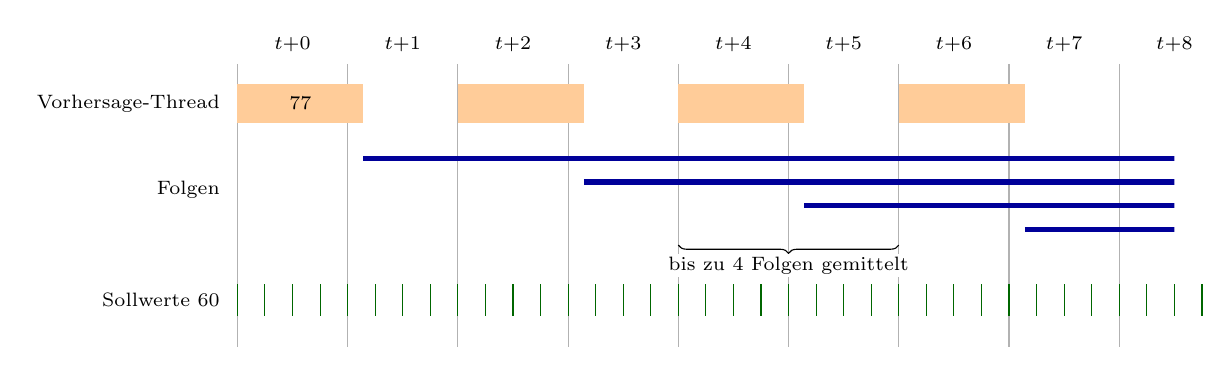
\begin{tikzpicture}[font=\small, x=1cm, y=1cm]
    % Taktachse
    \foreach \t in {0,...,8} {
      \draw[black!30] (\t*1.4,0) -- (\t*1.4,-3.6);
      \node[font=\scriptsize] at (\t*1.4+0.7,0.25) {$t{+}\t$};
    }
    \node[anchor=east, font=\scriptsize] at (-0.1,-0.5) {Vorhersage-Thread};
    \node[anchor=east, font=\scriptsize] at (-0.1,-1.6) {Folgen};
    \node[anchor=east, font=\scriptsize] at (-0.1,-3.0) {Sollwerte \SI{60}{\hertz}};
    % Vorhersagen
    \foreach \s in {0,2,4,6} {
      \fill[orange!40] (\s*1.4,-0.75) rectangle (\s*1.4+1.6,-0.25);
    }
    \node[font=\scriptsize] at (0.8,-0.5) {\SI{77}{\milli\second}};
    % Folgen
    \begin{scope}
      \clip (0,-2.4) rectangle (11.9,-1.0);
      \foreach \s/\y in {0/-1.2, 2/-1.5, 4/-1.8, 6/-2.1} {
        \draw[blue!60!black, line width=2pt] (\s*1.4+1.6,\y) -- (\s*1.4+1.6+8*1.4,\y);
      }
    \end{scope}
    % Sollwerte
    \foreach \i in {0,...,35} { \draw[green!40!black] (\i*0.35,-3.2) -- (\i*0.35,-2.8); }
    \draw[decorate, decoration={brace, amplitude=3pt, mirror}] (5.6,-2.3) -- (8.4,-2.3)
      node[midway, below=3pt, font=\scriptsize, fill=white, inner sep=1pt] {bis zu 4 Folgen gemittelt};
  \end{tikzpicture}
  \caption[Taktschema der Ausführung]{Taktschema der Ausführung (schematisch). Alle zwei
  Takte startet eine Vorhersage im eigenen Thread; ihre Folge gilt ab ihrem Eintreffen. Für
  jeden Takt werden die vorliegenden Folgen gemittelt, und der Sollwertstrom mit
  \SI{60}{\hertz} läuft ununterbrochen.}
  \label{fig:takt}
\end{figure}

% ==============================================================================
\section{Sollwertübertragung}
\label{sec:sollwerte}

Die Policy gibt Gelenkstellungen im Takt von \SI{15}{\hertz} aus. Zwischen zwei Takten werden
je drei Zwischenwerte linear interpoliert und die Sollwerte mit \SI{60}{\hertz} über den Befehl
\code{servo_j} an die Steuerung gesendet. Bei der Aufnahme gilt dasselbe; Aufnahme und
Ausführung benutzen denselben Sollwertstrom.

\subsection{Latenz und abbrechende Bahnen}

\paragraph{Problem.} Am ersten Labortag (01.10.) brach die Aufnahme gegen die \ac{vm} immer
wieder ab: Der Arm blieb unterwegs stehen, die Steuerung meldete einen Verbindungsabbruch, und
die Episoden wurden wegen des Zeitbudgets verworfen.

\paragraph{Analyse.} Mit eigenen Werkzeugen für Aufruflatenz, Sollwerttakt und
Trajektorienpuffer wurde der Fehler eingegrenzt \quelle{Dokumentation/Taktzeit-und-RPC-Latenz.md}.
Ergebnis: Nicht die Steuerung war zu langsam, sondern der Laptop, auf dem die \ac{vm} lief, war
im Energiesparmodus gedrosselt. Mit voller Leistung lief derselbe Stand mit \SI{60}{\hertz}
fehlerfrei. Zwei weitere Befunde wirkten sich dauerhaft aus:
\begin{itemize}
  \item Der Zustand des Roboters wird seitdem lokal aus den Gelenkwinkeln berechnet statt
    über einen zweiten Aufruf an die Steuerung. Das spart einen Aufruf je Takt und beseitigt
    einen Zeitversatz zwischen Gelenkwinkeln und \ac{tcp}-Pose.
  \item Bei Override \num{0.2} begrenzte die Steuerung die Gelenkgeschwindigkeit unter die
    geplante; der Arm fiel immer weiter zurück. Daraus entstand die Prüfung auf Schleppfehler,
    die seitdem jede Aufnahme überwacht (\cref{sec:gueltigkeit}). Gleichzeitig wurde klar,
    dass das Tempo vom Planer und nicht vom Override bestimmt werden muss.
\end{itemize}

% ==============================================================================
\section{Zittern an der Anlage}
\label{sec:zittern}

\paragraph{Problem.} In der \ac{vm} lief die Ausführung über \code{servo_j} mit
\SI{60}{\hertz} ruhig. An der realen Anlage zitterte der Arm am 05.10.\ deutlich; das Bauteil
rutschte, und die Kamerastange schwang mit.

\paragraph{Ursache.} Die Steuerung rechnet \code{servo_j} intern als Strom mit
\SI{1}{\kilo\hertz}. Sie fährt jeden \SI{60}{\hertz}-Sollwert an und wartet dann auf den
nächsten. Es entsteht eine treppenförmige Bewegung, die Arm und Aufbau bei
\SIrange{7}{8}{\hertz} anregt (\cref{fig:spektrum}). In der \ac{vm} fehlt die Mechanik, die
diese Treppe in eine Schwingung umsetzt. Gemessen wurde die Schwingung mit dem
Beschleunigungssensor eines Smartphones am Unterarm des Roboters, als Effektivwert der
Beschleunigung oberhalb von \SI{5}{\hertz}.

\begin{figure}[htbp]
  \centering
  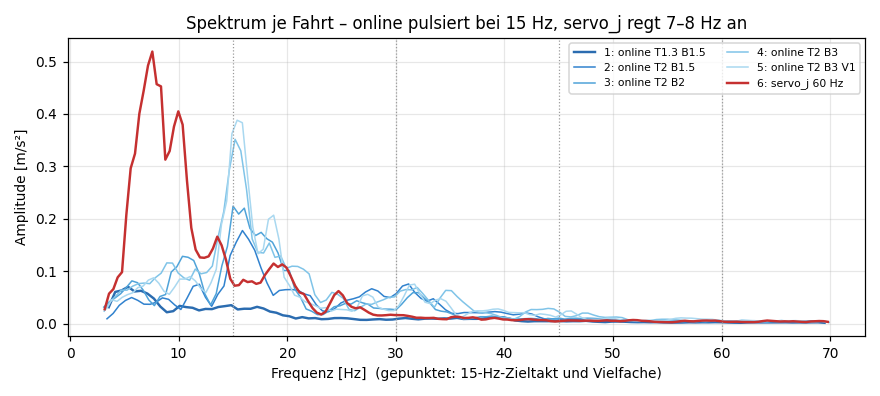
\includegraphics[width=\textwidth]{m4/03_handy_spektrum.png}
  \caption[Spektrum der Beschleunigung am Unterarm]{Spektrum der Beschleunigung am Unterarm
  je Fahrt. Rot: \code{servo_j} mit \SI{60}{\hertz}; blau: Varianten mit Interpolation in der
  Steuerung (\code{movelinear_online}).}
  \label{fig:spektrum}
\end{figure}

\paragraph{Untersuchte Lösungen.} \Cref{tab:zittern} fasst die Wege zusammen.
\begin{table}[htbp]
  \centering
  \caption{Untersuchte Ausführungsarten gegen das Zittern}
  \label{tab:zittern}
  \small
  \begin{tabularx}{\textwidth}{@{}>{\raggedright\arraybackslash}p{36mm} X X@{}}
    \toprule
    Ausführungsart & Vorteil & Nachteil \\
    \midrule
    höhere Rate von \code{servo_j} & kleinere Stufen & Laptop schafft sie über NeuraPy
      nicht stabil \\
    Bahnpuffer der Steuerung & Steuerung fährt glatt & in der vorhandenen Version nicht
      verfügbar \\
    \code{movelinear_online} (Steuerung interpoliert, 15 Ziele/s) & Schwingung
      \SI{-76}{\percent} & in Drehungen bis \SI{49}{\milli\metre} neben der Bahn und bis
      \SI{0.79}{rad} hinterher; kehrte \SI{27}{\milli\metre} über dem Greifpunkt um \\
    \code{servo_j} mit Override \num{0.5} & so ruhig wie ein Herstellerprogramm, Bahn
      $\le$ \SI{1.2}{\milli\metre} & Steuerung folgt etwa \SI{0.09}{\second} verzögert \\
    \bottomrule
  \end{tabularx}
\end{table}

\paragraph{Entscheidung.} Zunächst wurde \code{movelinear_online} gewählt, weil es die
Schwingung am stärksten senkte. Die Nachrechnung zeigte aber, dass der Arm damit in Kurven so
weit hinter der Sollbahn lag, dass die Schleppfehlerprüfung der Aufnahme und die
Sicherheitsprüfung der Ausführung jede Fahrt abgebrochen hätten. Für die Datenpaare ist das
grundsätzlich: Zustand und Sollstellung müssen zueinander passen. Am Labortag vom 19.10.\
bestätigte sich die Alternative: Mit \code{servo_j} und Override \num{0.5} führt die
Steuerung die Sollwerte weicher nach. Die Schwingung lag bei
\SIrange{0.19}{0.20}{\metre\per\second\squared} statt \SI{1.74}{\metre\per\second\squared}, also
auf dem Niveau eines Programms am Bedienhandgerät
(\SIrange{0.16}{0.18}{\metre\per\second\squared}, \cref{fig:h1}). Die Bahn wich höchstens
\SI{1.2}{\milli\metre} ab, und die Fahrzeit blieb gleich. Seitdem gilt \code{servo_j} mit
Override \num{0.5} für Aufnahme und Ausführung.

\begin{figure}[htbp]
  \centering
  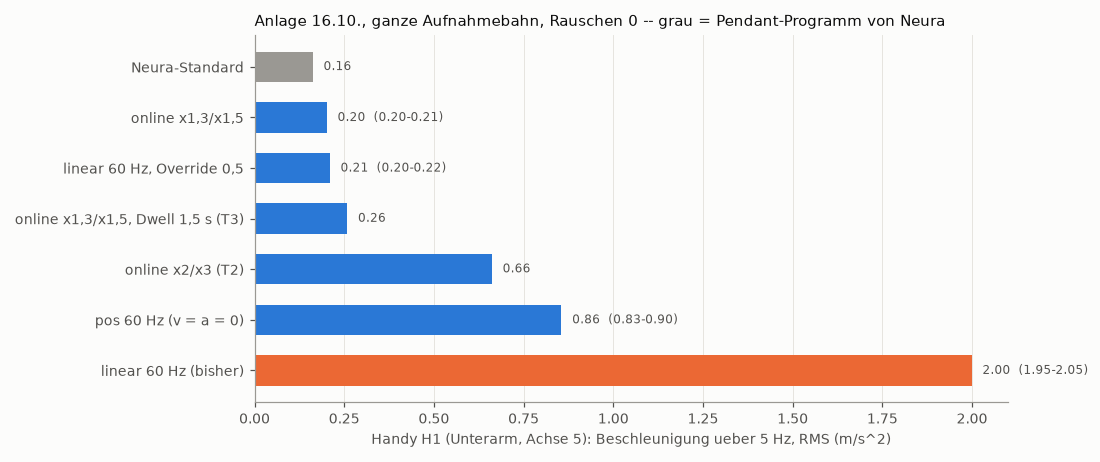
\includegraphics[width=\textwidth]{m4/13_labortag16_h1.png}
  \caption[Schwingung am Unterarm je Ausführungsart]{Schwingung am Unterarm über die ganze
  Aufnahmebahn je Ausführungsart (Effektivwert oberhalb \SI{5}{\hertz}, ohne Rauschen). Grau:
  Programm am Bedienhandgerät zum Vergleich.}
  \label{fig:h1}
\end{figure}

\todo[inline]{Override \num{0.5} mit dem Betreuer abstimmen und hier vermerken.}

Die ausführliche Untersuchung mit allen Messreihen steht in
\code{Dokumentation/Zittern-an-der-Anlage.md}; die Rohdaten liegen unter \code{Berichte/}.

% ==============================================================================
\section{Erfolgs- und Abbruchkriterium}
\label{sec:erfolg}

Die Fahrt gilt als erfolgreich beendet, wenn die Gelenke fünf Takte lang höchstens
\SI{0.02}{rad} von der Endstellung der Aufnahme entfernt sind und der Greifer geschlossen ist,
frühestens nach der halben typischen Episodenlänge. Die Stellung allein reicht nicht: In der
Simulation lag ein Zwischenpunkt auf dem Weg an derselben Stelle wie der Endpunkt, und ohne
Greiferbedingung wurde eine Fahrt mitten in der Bahn als fertig gewertet.

Früher wurde zusätzlich der Abstand zum Greifpunkt der Aufnahme bewertet. Bei wechselnden
Objektlagen ist das nicht mehr sinnvoll; dieser Wert ist nur noch Information. Abgebrochen
wird nach dem \num{1.5}-Fachen der längsten Episode, bei verletzter Sicherheitsprüfung
(\cref{ch:sicherheit}) oder wenn keine Vorhersage mehr rechtzeitig vorliegt.

Für Versuche mit bekannter Objektlage gibt es einen Probegriff: Die Policy fährt selbst, die
Lage ist aber wie bei der Aufnahme bekannt. Ziele, die tiefer als ein einstellbarer Abstand
über dem Bauteil liegen (Standard \SI{25}{\milli\metre}), werden abgelehnt. So lässt sich
prüfen, wohin die Policy greifen würde, ohne dass sie auf das Bauteil oder den Tisch fährt.

\paragraph{Protokoll.} Jede Fahrt wird mit allen Takten gespeichert: Zustand, Sollwerte, rohe
Vorhersagen, Vorhersagezeit, Verzug der Folgen, gekappte Takte und Abbruchgrund. Eine
Live-Ansicht zeigt während der Fahrt die Kamerabilder, die Spur des \ac{tcp} und die gerade
gemittelten Vorhersagen.
